
\renewcommand*\thesection{\arabic{section}}
\setcounter{section}{0}%更改chapter的计数器值
%\numberwithin{equation}{chapter}%公式计数器从属于节计数器
\numberwithin{equation}{section}%公式计数器从属于节计数器
\numberwithin{figure}{chapter}%图计数器从属于节计数器
%\renewcommand*\thefigure{\arabic{section}}
\setcounter{chapter}{0}


\chapter[瞬子]{瞬子\footnote{基于Sidney Coleman, {\textit{The Uses of Instantons}}.}}

\section{简介} \label{instanton:sec1}

考虑四维闵可夫斯基空间中的单个标量场, 其拉格朗日量是
\begin{equation}
    \mathscr{L}=\tfrac{1}{2}\partial_{\mu}\phi \partial^{\mu}\phi
    -\tfrac{1}{2}m^{2}\phi^{2}-g^{2}\phi^{4} \:.
\end{equation}
对于经典物理, $g$是无关参量. 可以定义
\begin{equation}
    \phi'=g\phi\:.
\end{equation}
写成$\phi'$, 
\begin{equation}
    \mathscr{L}=\frac{1}{g^{2}}\Bigl(\tfrac{1}{2}\partial_{\mu}\phi' \partial^{\mu}\phi'
    -\tfrac{1}{2}m^{2}\phi'^{2}-\phi'^{4} \Bigr)\:.
\end{equation}
因此场方程中没有$g$; 如果对任何正的$g$解出了这个理论, 就对其它所有正的$g$解出了这个理论; 所以$g$是无关的. 看到这点的另一个方法是: $g$在经典物理中是{\kaishu{有}}量纲的, 所以可被选为1.

在量子物理中, 由于引入了新常数$\hbar$, $g${\kaishu{是}}相关的, 而重要的物理量是
\begin{equation}
    \mathscr{L}/\hbar = \frac{1}{g^{2}\hbar}\Bigl(\tfrac{1}{2}\partial_{\mu}\phi' \partial^{\mu}\phi'
    -\tfrac{1}{2}m^{2}\phi'^{2}-\phi'^{4} \Bigr) \:.
\end{equation}
我们在这个表达式中看到, 相关(无量纲)参量是$g^{2}\hbar$, 因此半经典近似, 即小$\hbar$近似, 等同于弱耦合近似, 也就是小$g$近似.

我们有一个足以胜任的小耦合近似微扰论吗? 答案是否定的; 有许多有趣的现象在耦合常数很小时发生了但微扰论并不足以解释它们.

看到这点的最简单方法是从场论退回到力学. 考虑在一维势下运动的质量为1的粒子,
\begin{equation}
    L=\tfrac{1}{2}\dot{x}^{2}-V(x;g) \:, 
\end{equation}
其中
\begin{equation}
    V(x;g)=\frac{1}{g^{2}} F(gx) \:,
\end{equation}
而函数$F$的Taylor展开中的领头项是$x^{2}$阶的. 我们来考虑穿越势垒的跃迁现象(见图\ref{instantonfig1}). 
\begin{figure}[h]
    \centering
    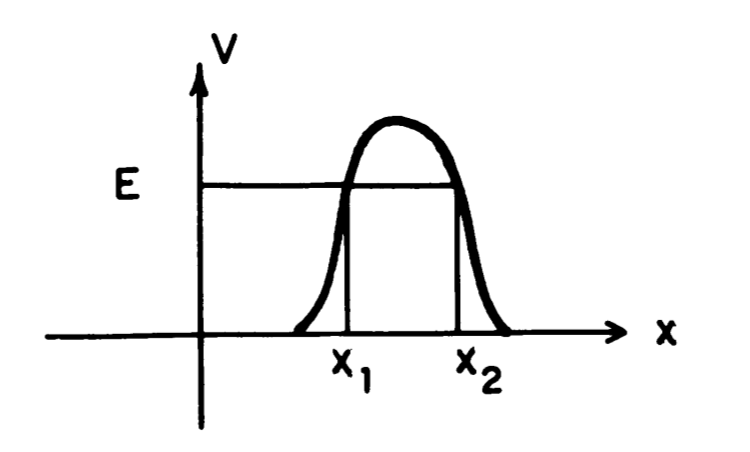
\includegraphics[width=0.6\textwidth]{instantonfig1.jpeg}
    \caption{ \label{instantonfig1}}
  \end{figure}

我们都知道这个跃迁振幅服从WKB公式
\begin{equation}
    \bigl\lvert T(E)\bigr\rvert =\exp\biggl(-\frac{1}{\hbar}\int_{x_{1}}^{x_{2}}\dif x\: \sqrt{2(V-E)}\biggr)[1+O(\hbar)] \:, \label{instanton1.7}
\end{equation}
其中$x_{1}$和$x_{2}$使得这个区域内的$V(x)$大于$E$. 
\begin{tcolorbox}
    一个非常简单的解释: 波函数可以近似写为$\exp(\mi p x/\hbar)$, 而$E=\frac{1}{2}p^{2}+V$, 所以在$E<V$时, $p=\mi\sqrt{2(V-E)}$, 波函数指数衰减.
\end{tcolorbox}
然而, 这个势垒隧穿在微扰论的任何阶都没有看到, 这是因为方程\eqref{instanton1.7}比$\hbar$的任意幂次都衰减的快, 因此也就比$g$的任意幂次都衰减得快.

在量子场论中, 尤其是量子色动力学中, 有类似于量子力学中的隧穿现象的效应, 这也就是所谓的瞬子.

{\heiti{符号说明}}: 时空特征是$({+}{-}{-}{-})$, $x^{0}$是时间坐标, $g_{\mu\nu}$是时空度规, $x^{4}=-\mi x^{0}$是到欧几里得时空的延拓.

\section{粒子力学中的瞬子和弹跳} \label{instanton:sec2}

\subsection{欧几里得泛函积分} \label{instanton:sec2.1}

在本节我们继续处理单位质量的无自旋粒子在一维势下运动的理论:
\begin{equation}
    H = \frac{p^2}{2} + V(x) \:. \label{instanton2.1}
\end{equation}
这是一个量子力学问题, 但我们不采用处理这类问题的标准方法, 而是容易推广到量子场论的方法.

我们的基本工具是Feynman历史求和的欧几里得版:
\begin{equation}
    \langle x_{\text{f}} \vert \me^{-HT/\hbar} \vert x_{\text{i}}\rangle =N \int [\dif x]\, \me^{-S/\hbar} \:. \label{instanton2.2}
\end{equation}
方程\eqref{instanton2.2}左边的$\lvert x_{\text{i}}\rangle$和$\lvert x_{\text{f}}\rangle$是位置本征态, $H$是哈密顿量, 而$T$是一个正数. 利用能量本征态
\begin{equation}
    H\vert n \rangle = E_{n} \vert n\rangle \label{instanton2.3}
\end{equation}
展开方程\eqref{instanton2.2}左边, 那么就有
\begin{equation}
    \langle x_{\text{f}} \vert \me^{-HT/\hbar} \vert x_{\text{i}}\rangle 
    = \sum_{n}\me^{-E_{n}T/\hbar}  \langle x_{\text{f}} \vert n\rangle \langle n \vert x_{\text{i}}\rangle  \:. \label{instanton2.4}
\end{equation}
这个展开在大$T$时的领头项给出了能量最低的本征态的能量和波函数.

在方程\eqref{instanton2.2}右边, $N$是归一化常数, $S$是欧几里得作用量
\begin{equation}
    S=\int_{-T/2}^{T/2} \dif t\:\biggl[\frac{1}{2}\biggl(\frac{\dif x}{\dif t}\biggr)^{2}+V\biggr] \:, \label{instanton2.5}
\end{equation}
而$[\dif x]$代表对所有满足边界条件$x(-T/2)=x_{\text{i}}$和$x(T/2)=x_{\text{f}}$的函数$x(t)$积分. 更具体一些, 如果$\overline{x}$是满足边界条件的任意函数, 那么满足边界的一般函数可以写成
\begin{equation}
    x(t)=\overline{x}(t)+\sum_{n}c_{n}x_{n}(t) \:, \label{instanton2.6}
\end{equation}
其中$x_{n}$是在边界处为零的实正交函数完备集,
\begin{subequations}\label{instanton2.7}
    \begin{gather}
        \int_{-T/2}^{T/2} \dif t\: x_{n}(t)x_{m}(t) = \delta_{nm} \:, \label{instanton2.7a} \\
        x_{n}(\pm T/2)=0 \:.  \label{instanton2.7b}
    \end{gather}
\end{subequations}
这样, 测度就定义成
\begin{equation}
    [\dif x] = \prod_{n} (2\pi\hbar)^{-1/2} \dif c_{n} \:. \label{instanton2.8}
\end{equation}
(这里的归一化常数$N$依赖于测度的定义, 但是归一化常数会抵消, 所以不需要它的准确定义.)

方程\eqref{instanton2.2}右边可以用半经典(小$\hbar$)极限计算. 在这个情况下, 泛函积分由$S$的稳定点主导. 简单起见, 我们假定只有一个这样的稳定点, 我们将其记为$\overline{x}$, 它满足牛顿方程
\begin{equation}
    \frac{\delta S}{\delta x}\biggr\vert_{x=\overline{x}} = 
    -\frac{\dif^{2}\overline{x}}{\dif t^{2}} + V'(\overline{x}) = 0 \label{instanton2.9}
\end{equation} 
其中加撇号代表对$x$的导数. 更进一步, 我们令$x_{n}$是$S$在$\overline{x}$处的二阶变分导数的本征函数,
\begin{equation}
    -\frac{\dif^{2} x_{n}}{\dif t^{2}} + V''(\overline{x})x_{n} = \lambda_{n}x_{n} \:. \label{instanton2.10} 
\end{equation}
那么, 在小$\hbar$极限下, 这个积分变成高斯积分的乘积, 所以有
\begin{align}
    \langle x_{\text{f}} \vert \me^{-HT/\hbar} \vert x_{\text{i}}\rangle 
   & = N \me^{-S(\bar{x})/\hbar}\prod_{n}\lambda_{n}^{-1/2}[1+O(\hbar)] \nonumber \\
   &= N \me^{-S(\bar{x})/\hbar}\Bigl[\det\bigl(-\partial_{t}^{2}+V''(\overline{x})\bigr)\Bigr]^{-1/2}[1+O(\hbar)] \:. \label{instanton2.11}
\end{align}
如果有数个稳定点, 一般需要求和.
\begin{tcolorbox}
    这里解释一下方程\eqref{instanton2.10}和\eqref{instanton2.11}, 在$\overline{x}$附近展开$S$, 并设微扰为$\eta$, 那么
    \begin{align*}
        \delta S&= S(\overline{x}+\eta)-S(\overline{x}) 
        = \int \dif t\, \Bigl(\tfrac{1}{2}\bigl(\dot{\overline{x}}+\dot{\eta}\bigr)^{2}+V(\overline{x}+\eta)-\tfrac{1}{2}\dot{\overline{x}}^{2}-V(\overline{x})\Bigr) \\
        &=\int \dif t\,\Bigl(\dot{\overline{x}}\dot{\eta}- V'(\overline{x})\eta+\tfrac{1}{2}\dot{\eta}^{2}+\tfrac{1}{2}V''(\overline{x})\eta^{2}+O(\eta^{2})\Bigr)
        =\frac{1}{2}\int \dif t\, \eta(-\partial_{t}^{2}+V'')\eta
    \end{align*}
在最后一个等号这里使用了牛顿方程\eqref{instanton2.9}, 分部积分并忽略了$\eta$的高阶项. 

用$(-\partial_{t}^{2}+V'')$的本征函数完备集$\{x_{n}\}$展开$\eta=\sum c_{n}x_{n}$, 利用方程\eqref{instanton2.7}就得到了
\begin{equation*}
    \delta S= \frac{1}{2} \lambda_{n}c_{n}^{2}
\end{equation*}
那么
\begin{align*}
    N \int [\dif x]\, \me^{-S/\hbar}&=N \me^{-S(\overline{x})/\hbar} \int [\dif x]\, \me^{-\delta S/\hbar} \\
    &=N \me^{-S(\overline{x})/\hbar} \int \prod_{n} (2\pi\hbar)^{-1/2} \dif c_{n}\:\me^{-\frac{1}{2} \lambda_{n}c_{n}^{2}/\hbar}
    =N \me^{-S(\overline{x})/\hbar}\prod_{n} \lambda_{n}^{-1/2} .
\end{align*}
\end{tcolorbox}

根据方程\eqref{instanton2.9}, 能量是
\begin{equation}
    E=\frac{1}{2}\biggl(\frac{\dif\overline{x}}{\dif t}\biggr)^{2} - V(\overline{x})
\end{equation}
这可以用来决定方程\eqref{instanton2.9}的解的定性性质.

\begin{figure}[h]
    \centering
    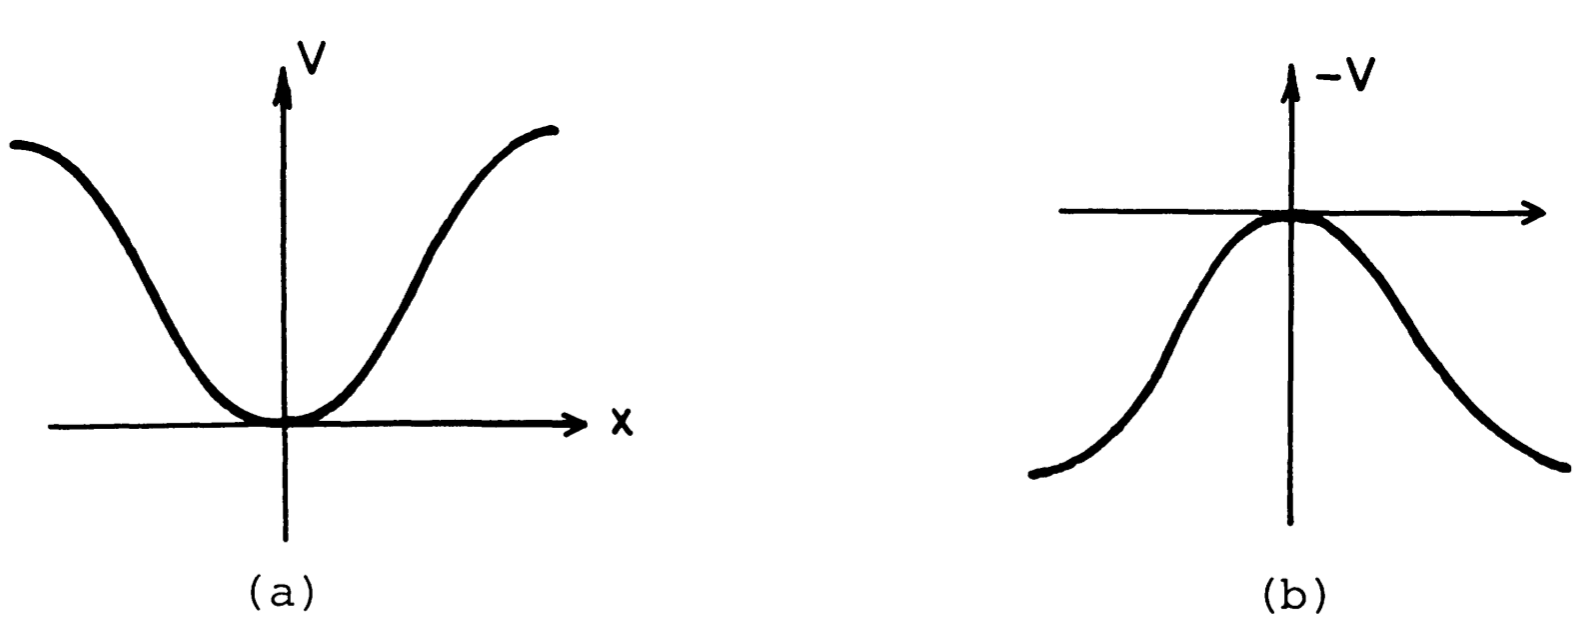
\includegraphics[width=0.8\textwidth]{instantonfig2.jpeg}
    \caption{ \label{instantonfig2}}
  \end{figure}
作为一个简单例子, 考虑图\ref{instantonfig2}(a)中的势能. 选择$x_{\text{i}}=x_{\text{f}}=0$. 方程\eqref{instanton2.9}满足边界条件的解显然是
\begin{equation}
    \overline{x}=0 . \label{instanton2.13}
\end{equation}
对于这个解, $S(\overline{x})=0$. 那么, 从方程\eqref{instanton2.11}
\begin{equation}
    \langle 0 \vert \me^{-HT/\hbar} \vert 0\rangle = 
    N[\det(-\partial_{t}^{2}+\omega^{2})]^{-1/2}[1+O(h)] \:, \label{instanton2.14}
\end{equation}
其中
\begin{equation}
    \omega^{2}=V''(0) \:. \label{instanton2.15}
\end{equation}

可以证明, 对于很大的$T$,
\begin{equation}
    N[\det(-\partial_{t}^{2}+\omega^{2})]^{-1/2} \simeq \biggl(\frac{\omega}{\pi\hbar}\biggr)^{1/2}\me^{-\omega T/2}.  \label{instanton2.16}
\end{equation}
根据方程\eqref{instanton2.4}, 基态能量是
\begin{equation}
    E_{0}=\frac{1}{2}\omega\hbar[1+O(\hbar)] \:. \label{instanton2.17}
\end{equation}
同理, 基态粒子处在原点的几率是
\begin{equation}
     \bigl\lvert \langle x{=}0 \vert n{=}0 \rangle \bigr\rvert^{2} =
     (\omega/\pi\hbar)^{1/2}[1+O(\hbar)] .
\end{equation}

这些当然是正确的半经典结果. 在小$\hbar$极限下, 粒子处在位于原点的谐振子基态中, 能量就是谐振子的基态能量.

\begin{tcolorbox}[breakable]
    推导方程\eqref{instanton2.16}的两种方法:

    (1)蛮干法(Poor man's way): 求解如下微分方程
\[
 (-\partial_{t}^{2}+\omega^{2})f= \lambda_{n}f
\]
由于$f$要满足边界条件$f(\pm T/2)=0$, 所以$\lambda_{n}>\omega^{2}$, 并要满足
\[
 \sqrt{\lambda_{n}-\omega^{2}} = \frac{n\pi}{T}    
\]
那么根据方程\eqref{instanton2.11}, 
\begin{align*}
    [\det(-\partial_{t}^{2}+\omega^{2})]^{-1/2}
    =\prod_{n}\biggl(\frac{n^{2}\pi^{2}}{T^{2}}+\omega^{2}\biggr)^{-1/2}
\end{align*}
上式需要重整化, 除以一个不依赖于$\omega$的无限大常数$[\det(-\partial_{t}^{2})]^{-1/2}$, 得到
\begin{align*}
    [\det(-\partial_{t}^{2}+\omega^{2})]^{-1/2}&=\prod_{n}\Biggl(
        1+ \biggl(\frac{\omega T}{n\pi}\biggr)^{2}\Biggr)^{-1/2} \\
        &= \biggl(\frac{\sinh(\omega T)}{\omega T}\biggr)^{-1/2}
\end{align*}
在$T$很大时, $\sinh(\omega T)\simeq \me^{\omega T}$. 常数$N$可以通过考虑自由粒子来决定, 这里不再赘述.

(2) Coleman的方法, 根据定义
\[
\det(-\partial_{t}^{2}+W)=\prod_{n}\lambda_{n}    
\]
其中$\lambda_{n}$是算符$(-\partial_{t}^{2}+W)$的本征值, 那么$(-\partial_{t}^{2}+W-\lambda)$的本征值是$\lambda_{n}-\lambda$. 这样就有
\[
\frac{\det(-\partial_{t}^{2}+W^{(1)}-\lambda)}{\det(-\partial_{t}^{2}+W^{(2)}-\lambda)}  = \frac{\psi_{\lambda}^{(1)}(T/2)}{\psi_{\lambda}^{(2)}(T/2)}  .
\]
这里$\psi$满足
$(-\partial_{t}^{2}+W^{(i)})\psi_{\lambda}^{(i)}=\lambda \psi_{\lambda}^{(i)}$以及边界条件$\psi_{\lambda}(-T/2)=0$和$\dot{\psi}_{\lambda}(-T/2)=1$. 显然$\psi_{\lambda}^{(i)}$只有$\lambda=\lambda_{n}$时满足边界条件$\psi_{\lambda}^{(i)}(\pm T/2)=0$. 将上式左右两边视为$\lambda$的函数, 那么左右两边就有相同的零点和极点, 所以相等.

由此可得
\[
    \frac{\det(-\partial_{t}^{2}+W)}{\psi_{0}(T/2)} =\text{常数} = \pi\hbar N^{2} 
\]
其中$N$是一个常数. (这也是Coleman对$N$的定义.) 对于$W=\omega^{2}$, 可以解出
\[
\psi_{0}=\omega^{-1} \sinh \omega(t+T/2)\:,   
\]
进而也就得到了方程\eqref{instanton2.16}

\end{tcolorbox}


\subsection{双井与瞬子} \label{instanton:sec2.2}

我们现在转向不那么平庸的问题, 图\ref{instantonfig3}(a)所示的双井. 假定势是偶函数, $V(x)=V(-x)$, 它的最小值点记为$\pm a$. 选择一个常数, 使得$V$的最小值是0, 并将$V''(\pm a)$记为$\omega^{2}$
\begin{figure}[h]
    \centering
    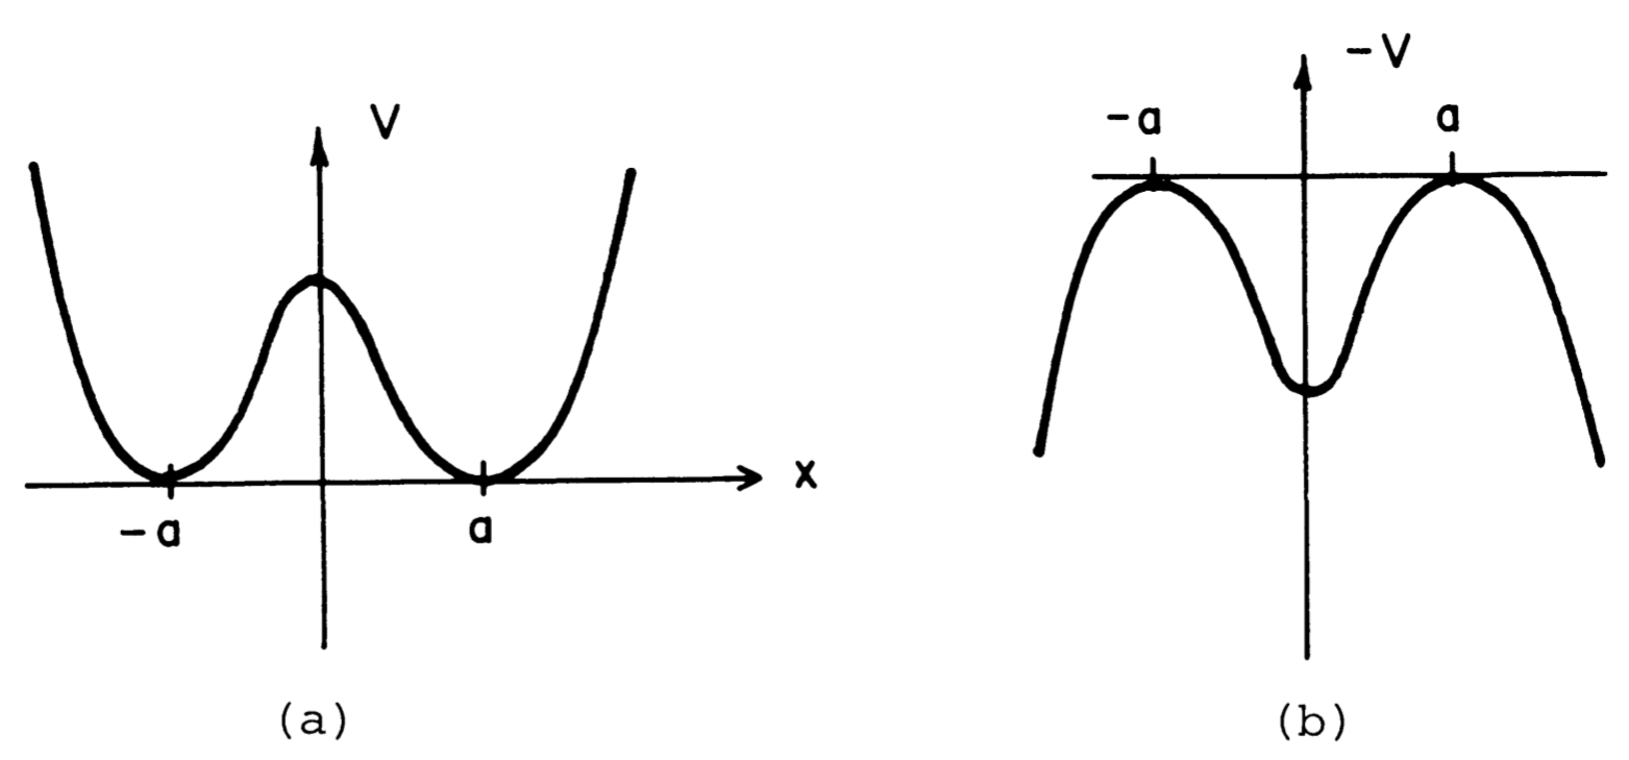
\includegraphics[width=0.8\textwidth]{instantonfig3.pdf}
    \caption{ \label{instantonfig3}}
\end{figure}

我们将尝试计算
\begin{subequations}
    \begin{align}
        \langle {-}a \vert \me^{-HT} \vert {-}a \rangle &= \langle a \vert \me^{-HT} \vert a \rangle \:, \label{instanton2.19a}\\ 
        \langle a \vert \me^{-HT} \vert {-}a \rangle &= \langle {-}a \vert \me^{-HT} \vert a \rangle \:,\label{instanton2.19b}
    \end{align}
\end{subequations}
方法是通过半经典极限方程\eqref{instanton2.11}来近似泛函积分. 和前面一样, 先求解与边界条件相容的经典欧几里得运动方程, \eqref{instanton2.9}. 

当然, 两个这样的解是粒子待在两个井底(或者说图\ref{instantonfig3}(b)的两个山顶). 然而还有另一种有趣的解, 在$-T/2$时待在其中一个山顶, 然后在$T/2$时跑到另一个山顶.
由于我们最后会把$T$取为无穷大, 我们将专注于这个极限下的解形式, 即粒子在无穷远的过去从一个山顶离开, 然后在无穷远的未来达到另一个山顶. 在这个情况下, 运动方程的解的能量为零; 
所以
\begin{equation}
    \dif x/\dif t =\sqrt{2V}. \label{instanton2.20}
\end{equation}
等效地有
\begin{equation}
    t= t_{1}+\int_{0}^{x}\dif x' \: (2V)^{-1/2} \:, \label{instanton2.21}
\end{equation}
其中$t_{1}$是积分常数, $x(t_{1})$为零.

\begin{figure}[h]
    \centering
    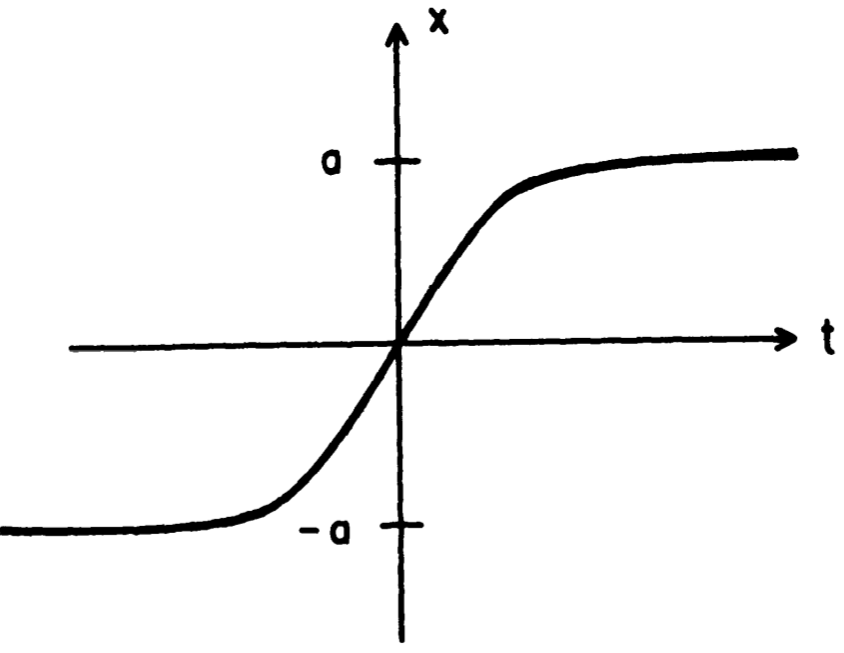
\includegraphics[width=0.5\textwidth]{instantonfig4.jpeg}
    \caption{ \label{instantonfig4}}
  \end{figure}

解的图示参看图\ref{instantonfig4}; 它被称为``中心在$t_{1}$的瞬子''. 瞬子这一词汇是't Hooft发明的. 灵感来源于它们的数学结构十分类似于所谓的孤子(solitons)或鼓包(lump), 
经典场论的类粒子解: 因此称为``-子''. 然而, 不像鼓包, 它们在时间(尽管是欧几里得时间)中是局域的: 因此是``瞬-''. 由于相同的原因, Polyakov称其为``赝粒子(pseudoparticle)'', 也见于文献.

当然, 我们可以也可以构建从$a$到${-}a$的解, 将方程\eqref{instanton2.21}中的$t$换为$-t$即可; 它们被称为``反瞬子''.

这些解有两个很重要的性质:
\begin{enumerate}
    \item 从方程\eqref{instanton2.20}可以导出瞬子(或反瞬子)作用量的一个简单表达式
    \begin{equation}
        S_{0}=\int \dif t\:\bigl[\tfrac{1}{2}\dot{x}^{2}+V\bigr] =\int \dif t \: \dot{x}^{2} = \int_{-a}^{a}\dif x\:\sqrt{2V} \:. \label{instanton2.22}
    \end{equation}
    注意这与势垒隧穿公式\eqref{instanton1.7}中出现的积分相同. 我们会在后面看到这不是个巧合.
    \item 对于大$t$, $x$趋于$a$, 方程\eqref{instanton2.20}可以近似为
    \begin{equation}
        \dot{x} = \omega(a-x) \:. \label{instanton2.23}
    \end{equation}
    因此, 对于大$t$,
    \begin{equation}
        (a-x) \propto \me^{-\omega t} \:. \label{instanton2.24}
    \end{equation}
    因此瞬子是一个非常定域的物体, 它的尺寸大约是$1/\omega$阶的.
\end{enumerate}

这是十分重要的, 因为这意味着: 当$T$很大时, 瞬子和反瞬子不仅是运动方程的近似解; 相距甚远的瞬子和反瞬子串联而成的场构型也是近似解. 

泛函积分将通过对所有这样的构型求和计算, 其中每个构型有$n$个物体(瞬子或反瞬子), 中心处在$t_{1},\ldots,t_{n}$, 其中
\begin{equation}
    T/2>t_{1}>\cdots>t_{n}>-T/2\:. \label{instanton2.25}
\end{equation}

图\ref{instantonfig5}展示了这样一个构型. $T$相比于瞬子尺寸要大很多; 因此图\ref{instantonfig4}的光滑曲线在图5的尺度上就变成了尖锐的跃变. 

\begin{figure}[h]
    \centering
    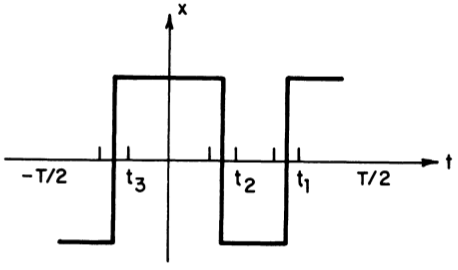
\includegraphics[width=0.6\textwidth]{instantonfig5.jpeg}
    \caption{ \label{instantonfig5}}
  \end{figure}

现在是计算:
\begin{enumerate}
    \item 对于$n$个相距甚远的物体, $S$就是$n S_{0}$. 要考虑到作用量在指数上.
    \item 泛函行列式的计算需要一些技巧. 我们把时间演化算符$\me^{-HT}$视为图\ref{instantonfig5}中时间轴上垂直线所标出的点之间的演化算符的乘积. 
    要不是存在含有瞬子和反瞬子的小区间, $V''$在整个时间上等于$\omega^{2}$, 因此我们所获得的结果与\ref{instanton:sec2.1}节中的单井势的结果相同, 
    \begin{equation}
        \biggl(\frac{\omega}{\pi\hbar}\biggr)^{1/2} \me^{-\omega T/2} \:. \label{instanton2.26}
    \end{equation}
    含有瞬子和反瞬子的小区间修正了这个公式. 因此我们得到
    \begin{equation}
        \biggl(\frac{\omega}{\pi\hbar}\biggr)^{1/2} \me^{-\omega T/2}K^{n} \:. \label{instanton2.27}
    \end{equation}
    其中$K$可以通过计算只有一个瞬子的情况得到.
    \item 我们必须要对瞬子中心所处的位置的积分:
    \begin{equation}
        \int_{-T/2}^{T/2} \dif t_{1}\int_{-T/2}^{t_{1}} \dif t_{2} \cdots \int_{-T/2}^{t_{n-1}} \dif t_{n} 
        =T^{n}/n! \:. \label{instaton2.28}
    \end{equation}
    \item 我们无法自由地分配瞬子和反瞬子. 例如, 如果我们从${-}a$出发, 那么第一个遇到的物体必然是瞬子, 下一个必然是反瞬子, 以此类推. 
    更进一步, 如果我们最后返回${-}a$, $n$必须是偶数. 同样, 如果我们最后停到了$a$, $n$必须是奇数. 
\end{enumerate}

因此,
\begin{equation}
    \langle{-}a\vert \me^{-HT/\hbar} \vert {-a}\rangle 
    =\biggl(\frac{\omega}{\pi\hbar}\biggr)^{1/2} \me^{-\omega T/2} 
    \sum_{\text{even }n} \frac{\bigl(K\me^{-S_{0}/\hbar}T\bigr)^{n}}{n!}[1+O(\hbar)] \:, \label{instanton2.29}
\end{equation}
而$\langle a\vert \me^{-HT/\hbar} \vert {-a}\rangle $由只对奇数$n$求和的相同表达式给出. 这些求和是平庸的:
\begin{equation}
    \langle \pm a\vert \me^{-HT/\hbar} \vert {-a}\rangle 
    =\frac{1}{2}\biggl(\frac{\omega}{\pi\hbar}\biggr)^{1/2} \me^{-\omega T/2}
    \Bigl[\exp\bigl(K\me^{-S_{0}/\hbar}T\bigr)\pm \exp\bigl(-K\me^{-S_{0}/\hbar}T\bigr)\Bigr] 
    \:, \label{instanton2.30}
\end{equation}
(从现在起将省略因子$[1+O(\hbar)]$.)

与方程\eqref{instanton2.4}比较, 我们现在有两种能量最底态, 其能量是
\begin{equation}
    E_{\pm} = \tfrac{1}{2}\hbar\omega \pm \hbar K \me^{-S_{0}/\hbar} \:. \label{instanton2.31}
\end{equation}
如果我们把这些本征态记为$\lvert + \rangle$和$\lvert - \rangle$, 我们看到
\begin{equation}
    \bigl \lvert \langle + \vert {\pm} a \rangle \bigr \rvert^{2} = \bigl \lvert \langle - \vert {\pm} a \rangle \bigr \rvert^{2} 
    =\langle a\vert -\rangle \langle - \vert {-}a\rangle =-\langle a\vert +\rangle \langle + \vert {-}a\rangle 
    =\frac{1}{2} \biggl(\frac{\omega}{\pi\hbar}\biggr)^{1/2} \:. \label{instanton2.32}
\end{equation}
当然, 它们是预期的结果: 能量本征态是中心在两个井底的谐振子态在空间上为偶或为奇的组合; 两个能量本征态的简并只被势垒隧穿破坏了(因此能量差正比于势垒隧穿因子$\me^{-S_{0}/\hbar}$), 而能量较低的态, 即我们记为$\lvert -\rangle$的那个, 在空间上为偶的组合. \\
\begin{remark}
设$\vert + \rangle= (m_{+}\lvert 0_{+}\rangle+n_{+}\lvert 0_{-}\rangle)/\sqrt{2}$和$\vert - \rangle= (m_{-}\lvert 0_{+}\rangle+n_{-}\lvert 0_{-}\rangle)/\sqrt{2}$, 其中$\lvert 0_{\pm}\rangle$是中心分别处在$\pm a$的谐振子态. 方程\eqref{instanton2.32}给出$m_{+}=-n_{+}$和$m_{-}=n_{-}$, 以及它们的范数为1.
\end{remark}

下个任务是计算$K$. 在计算之前, 我们先对所做的事情做一些评论:
\begin{enumerate}
    \item 实际上我们没有权利在方程\eqref{instanton2.31}中保留第二项. 不仅是因为它指数式小于第一项, 它也指数式得小于对第一项的未知$O(\hbar^{2})$修正. 然而这是对能量差$E_{+}-E_{-}$的领头阶修正; 一个更加严格的做法是仅在能量差的表达式中保留这一项, 而在单个能量的表达式中略去它.
    \item 我们的近似基于瞬子和反瞬子相距甚远的假定. 作为一个自洽性检验, 我们应该验证最后结果的主要部分来自于这样的构型. 
    
    这个检验很容易做. 对于固定的$x$, 指数系数$\sum x^{n}/n!$中的项随着$n$的增长而增长直到$n$到达$x$的量级, 在这之后, 开始快速衰减. 对方程\eqref{instanton2.29}中的求和应用这个性质, 我们看到重要的项是那些
    \begin{equation}
        n \lesssim KT \me^{-S_{0}/\hbar} \label{instanton2.33}
    \end{equation}
    的项. 这就是说, 对于小$\hbar$, 求和中重要的项是那些瞬子和反瞬子密度$n/T$是指数量级小数的项, 因此平均间隔非常大. 注意到这个平均间隔$K\me^{-S_{0}\hbar}$实际上独立于$T$; 我们的近似实际上是小$\hbar$近似; 只要$T$足够大, 这个条件就独立于$T$而成立.

    瞬子相距甚远这个近似被称为稀薄气体近似.
    \item 最后进一步解释下$S$的近似稳相点这个概念. 我们先来看单变量积分,
    \begin{equation}
        I=\int_{0}^{T} \dif t\: \me^{-S(t)/\hbar} \:, \label{instanton2.34}
    \end{equation}
    其中$S$是$t$的单调递减函数, 它的渐进值是$S(\infty)$. 因此这个被积函数在积分区域中没有稳相点. 然而对于小$\hbar$和大$T$, 很容易找到这个积分的如下近似形式
    \begin{equation}
        I\approx T \me^{-S(\infty)/\hbar} \:. \label{instanton2.35}
    \end{equation}
    大概地讲, 这个积分被无穷远处的稳相点所主导. 将这个现象推广到多维积分是直接的: 我们假定被积函数的图像有某种波谷; 沿着谷底的线会随着我们趋于无穷远而变平. 换言之, 在高维空间中有一条线, 使得被积函数在垂直于线的方向上在该线所处的位置达到最小值, 并在沿着这条线趋于无穷远时达到某个近似值. 当然这个线本身可以推广至超平面. ``近似稳相点''实际上就是这样的情况; 瞬子和反瞬子的所在就是沿着谷底的变量; $S$仅在它们趋于无穷远处变得稳定(并等于$nS_{0}$).
\end{enumerate}
\vspace{0.5cm}
现在我们来计算$K$.


\subsection{周期势}

\subsection{非稳态与弹跳}


\section{规范场论中的真空结构}

\subsection{冷饭}

\subsection{缠绕数}

\subsection{多个真空}

\subsection{瞬子: 一般情形}

\subsection{瞬子: 特殊情形}

\section{$1+1$维中的阿贝尔Higgs模型}

\section{$U(1)$问题的't Hooft解决方案}


\section{假时空的命运}